\chapter{Sprint 1 --- Données et gouvernance}

\section*{Introduction}
\addcontentsline{toc}{section}{Introduction}

Avant d'entraîner un modèle, il faut connaître les données sur lesquelles il apprendra. Le premier
sprint a donc porté sur le corpus : le rassembler, le décrire, mesurer ce qu'il vaut, puis le
préparer.

Nous présentons ici ce corpus : sa provenance, son contenu, ce que son analyse a révélé, les
corrections que nous lui avons apportées et les limites qui subsistent. La dernière section traite
du découpage entre entraînement et test. Elle occupe une place importante dans ce chapitre, car la
validité de tous les résultats rapportés aux chapitres~4 et~5 en dépend.

\section{Objectifs du sprint}

Le sprint poursuit cinq objectifs, récapitulés au tableau~\ref{tab:obj3}. Ils suivent le
séquencement de CRISP-DM exposé au chapitre~1 : comprendre les données avant de les préparer, et
les préparer avant d'entraîner quoi que ce soit.

\begin{table}[!htbp]
\centering
\styletableau
\caption{Objectifs du sprint 1 et livrables associés}
\label{tab:obj3}
\begin{tabular}{|Cp{0.8cm}|Lp{6.0cm}|Lp{4.4cm}|Lp{2.4cm}|}
\hline
\rowcolor{enteteTab}
\textbf{N\textsuperscript{o}} & \textbf{Objectif} & \textbf{Livrable} & \textbf{État} \\
\hline
1 & Décrire le corpus et mesurer sa qualité & Rapport de diagnostic et figures associées &
Atteint \\
\hline
2 & Situer le corpus par rapport à un jeu de données public & Comparaison structurelle et
lexicale & Atteint \\
\hline
3 & Définir des règles de nettoyage adaptées au vocabulaire informatique & Module de
prétraitement & Atteint \\
\hline
4 & Établir un découpage entraînement/test exempt de fuite & Jeux \texttt{train}, \texttt{test} et
\texttt{rag} & Atteint avec réserve \\
\hline
5 & Rendre la préparation reproductible & Pipeline de données versionné & Atteint \\
\hline
\end{tabular}
\end{table}

La réserve portée à l'objectif~4 s'explique à la section~\ref{sec:composition}. Le découpage
élimine bien la fuite que nous cherchions à supprimer, mais il produit un jeu de test dont la
couverture reste incomplète. Le protocole d'évaluation du chapitre~4 tient compte de ce défaut.

\section{Le jeu de données}

\subsection{Provenance et mode de collecte}

Le corpus provient de la liste SharePoint tenue par le service support, exportée au format CSV. Le
champ \texttt{Chemin d'accès} conserve l'emplacement d'origine de chaque enregistrement,
\texttt{sites/IT-Check/Lists/HelpDesk}, ce qui atteste la provenance sans dépendre d'une
déclaration.

L'export compte 1\,800 tickets créés entre le 1\textsuperscript{er} janvier 2025 et le
17 février 2026, soit quatorze mois d'activité et une moyenne de 129 tickets par mois. Ils émanent
de 202 demandeurs distincts répartis sur les huit filiales du groupe, et sont assignés à onze
intervenants, ce qui recoupe l'effectif du service décrit au chapitre~1.

Un défaut de saisie se voit dès l'ouverture du fichier. Le champ \texttt{Date de création} mélange
deux formats : 828 lignes au format ISO \texttt{AAAA-MM-JJ hh:mm:ss} et 972 au format français
\texttt{JJ/MM/AAAA hh:mm}. Une lecture qui n'essaierait qu'un seul format écarterait silencieusement
plus de la moitié des dates et fausserait toute statistique temporelle. Nous reconnaissons donc les
deux formats explicitement au chargement.

\subsection{Schéma et variable cible}

Chaque ticket est décrit par dix-huit champs. Le tableau~\ref{tab:schema} les regroupe par rôle
plutôt que dans l'ordre du fichier, afin de faire apparaître la structure de l'information.

\begin{table}[!htbp]
\centering
\styletableau
\caption{Organisation des dix-huit champs du jeu de données}
\label{tab:schema}
\begin{tabular}{|Bp{2.6cm}|Lp{5.2cm}|Lp{5.8cm}|}
\hline
\rowcolor{enteteTab}
\textbf{Groupe} & \textbf{Champs} & \textbf{Rôle dans le projet} \\
\hline
Identification & \texttt{ID}, \texttt{CID} & Clé du ticket et référence de configuration \\
\hline
Contenu & \texttt{Titre}, \texttt{Description} & Entrée textuelle des modèles \\
\hline
Classement & \texttt{Catégorie}, \texttt{Classification}, \texttt{Priorité} & \texttt{Catégorie}
est la variable cible ; les deux autres servent de contexte \\
\hline
Acteurs & \texttt{Demandeur}, \texttt{Filiale}, \texttt{Assigné~à} & Traçabilité de la demande et
de son traitement \\
\hline
Suivi & \texttt{STATUT}, \texttt{Date de création}, \texttt{Date de résolution} & Cycle de vie du
ticket \\
\hline
Résolution & \texttt{Résolution/Motif}, \texttt{Analyse}, \texttt{knowledge Base} & Matière de la
base de connaissances interrogée par le moteur RAG \\
\hline
Provenance & \texttt{Type d'élément}, \texttt{Chemin~d'accès} & Origine SharePoint de
l'enregistrement \\
\hline
\end{tabular}
\end{table}

La variable cible est le champ \texttt{Catégorie}, qui prend huit modalités : \emph{Microsoft},
\emph{Réseau}, \emph{Applicatifs}, \emph{Infrastructure}, \emph{Système}, \emph{Communication},
\emph{Sécurité} et \emph{Backup}. C'est le référentiel employé par le service, déjà introduit au
chapitre~1.

L'annotation elle-même est fiable. Aucun titre de ticket ne reçoit deux catégories différentes
selon les enregistrements : sur les 58 libellés distincts que compte le corpus, la correspondance
du titre vers la catégorie est une fonction, sans exception. Ce constat écarte d'emblée le bruit
d'étiquetage comme explication des performances observées au chapitre~4.

\subsection{Un jeu de données public pour situer le corpus}

Pour disposer d'un point de comparaison extérieur, nous avons chargé un jeu de données public de
tickets de support \cite{hfTickets}, filtré sur les enregistrements en langue anglaise, soit
11\,923 tickets décrits par quinze champs. Sa structure recoupe largement la nôtre, comme le montre
le tableau~\ref{tab:bench}.

\begin{table}[!htbp]
\centering
\styletableau
\caption{Correspondance entre le corpus \OTBS et le jeu de données public}
\label{tab:bench}
\begin{tabular}{|Bp{3.6cm}|Lp{4.2cm}|Lp{5.4cm}|}
\hline
\rowcolor{enteteTab}
\textbf{Corpus \OTBS} & \textbf{Jeu public} & \textbf{Rôle} \\
\hline
\texttt{Titre} & \texttt{subject} & Titre court \\
\hline
\texttt{Description} & \texttt{body} & Texte libre \\
\hline
\texttt{Catégorie} (8 classes) & \texttt{queue} (10 classes) & Cible de classification \\
\hline
\texttt{Classification} & \texttt{type} & Nature de la demande \\
\hline
\texttt{Priorité} & \texttt{priority} & Priorité déclarée \\
\hline
\texttt{Résolution/Motif} & \texttt{answer} & Réponse apportée \\
\hline
\end{tabular}
\end{table}

La langue et le domaine applicatif diffèrent trop pour que ce jeu serve à l'entraînement. Il sert
de repère, et livre au passage un chiffre réexploité plus loin. Le jeu public compte 10\,891 titres
distincts pour 11\,923 tickets, soit 91\,\% de titres uniques. Le nôtre en compte 58 pour 1\,800, soit 3\,\%. L'écart est
considérable pour deux corpus qui décrivent la même activité ; nous y revenons à la
section~\ref{sec:representativite}.

\section{Analyse exploratoire}

\subsection{Distribution des catégories}

La figure~\ref{fig:distcat} donne la répartition des 1\,800 tickets entre les huit catégories.

\begin{figure}[!htbp]
\centering
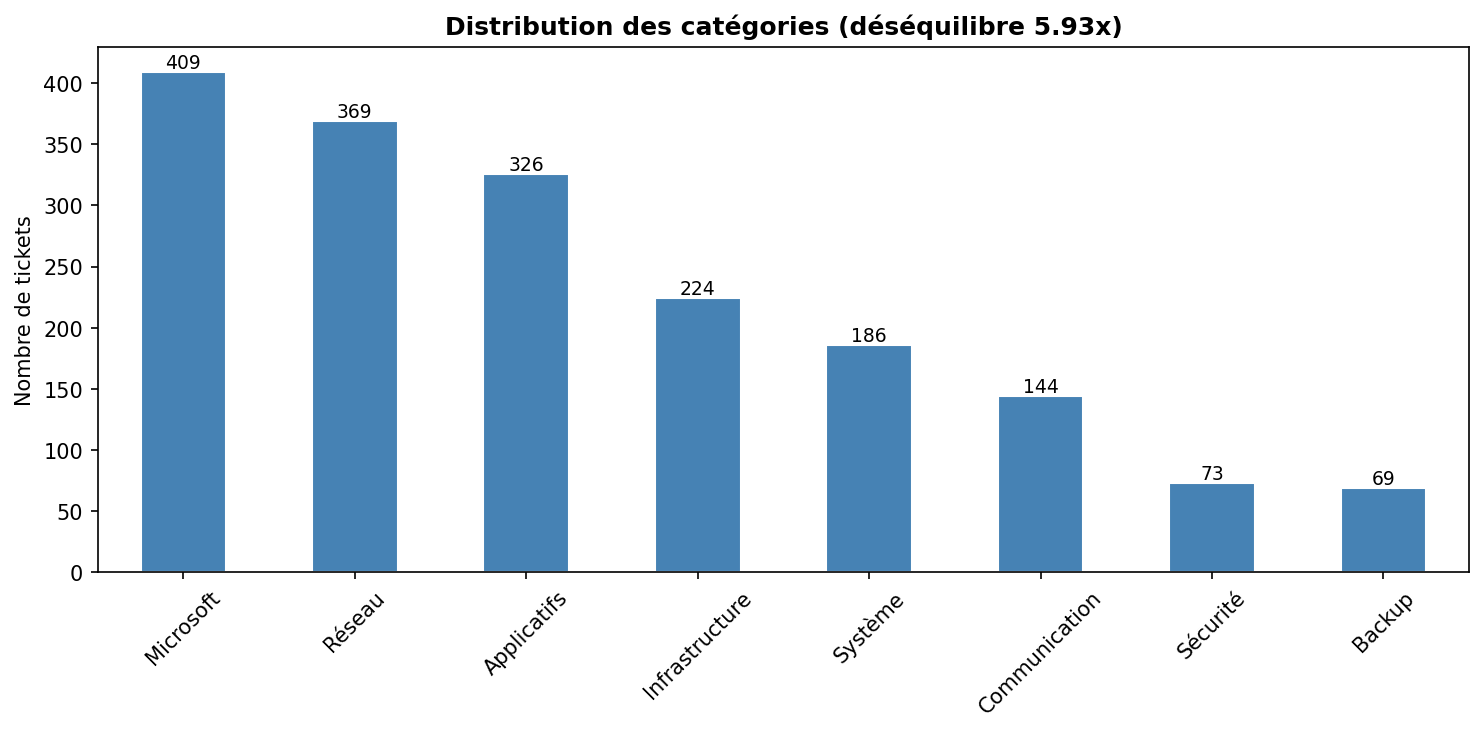
\includegraphics[width=0.94\textwidth]{ch03_distribution_categories.png}
\caption{Répartition des tickets par catégorie}
\label{fig:distcat}
\end{figure}

La distribution est nettement inégale. \emph{Microsoft} rassemble 409 tickets et \emph{Réseau} 369,
quand \emph{Sécurité} en compte 73 et \emph{Backup} 69. Le rapport entre la catégorie la plus
fréquente et la plus rare atteint 5,93. Les trois premières catégories concentrent à elles seules
1\,104 tickets, soit 61\,\% du corpus.

Ce déséquilibre est celui de l'activité réelle du service. Il pose en revanche une difficulté de
modélisation. Un classifieur entraîné sans précaution sur une telle
distribution apprend à privilégier les catégories abondantes ; il affiche alors une exactitude
globale élevée tout en échouant sur les catégories rares. Le problème est d'autant plus gênant que
\emph{Sécurité}, l'une des deux catégories les moins représentées, est celle dont une erreur de
classement coûte le plus cher au service. Nous traitons ce point au chapitre~4, par le choix de la
métrique et par la pondération des classes.

\subsection{Complétude des champs}

Douze des dix-huit champs sont renseignés sur la totalité des lignes, dont les quatre qui portent
l'information exploitée par les modèles : \texttt{Titre}, \texttt{Description}, \texttt{Catégorie}
et \texttt{knowledge Base}. Le tableau~\ref{tab:completude} recense les six champs incomplets.

\begin{table}[!htbp]
\centering
\styletableau
\caption{Champs incomplets et interprétation}
\label{tab:completude}
\begin{tabular}{|Bp{3.4cm}|Cp{2.0cm}|Lp{7.4cm}|}
\hline
\rowcolor{enteteTab}
\textbf{Champ} & \textbf{Manquant} & \textbf{Interprétation} \\
\hline
\texttt{Date de résolution} & 73,6\,\% & Manquant par construction : seuls les 476 tickets au
statut \emph{Résolu} en portent une \\
\hline
\texttt{CID} & 50,3\,\% & Référence de configuration renseignée au cas par cas, sans caractère
obligatoire \\
\hline
\texttt{Résolution/Motif} & 5,9\,\% & Traité par un repli sur \texttt{knowledge Base} dans le
moteur RAG \\
\hline
\texttt{Analyse} & 5,6\,\% & Champ de commentaire libre, facultatif \\
\hline
\texttt{Priorité} & 3,4\,\% & Non renseignée à la saisie \\
\hline
\texttt{Assigné à} & 3,1\,\% & Tickets non encore attribués au moment de l'export \\
\hline
\end{tabular}
\end{table}

Aucune de ces lacunes ne compromet le projet. Les deux taux les plus élevés s'expliquent par la
nature même des champs concernés, et les quatre autres restent sous 6\,\%. Le diagnostic du
chapitre~1 s'éclaire au passage : les canaux d'arrivée hétérogènes dégradaient la traçabilité en
amont de la liste SharePoint, mais le service remplissait correctement les enregistrements qui y
parvenaient.

\subsection{Longueur des textes et cycle de vie}

Les descriptions sont courtes et homogènes : de 23 à 46 mots, pour une médiane de 33 et une moyenne
de 33,1. Aucun ticket n'est vide, aucun n'est aberrant par la longueur. Les titres comptent de 2 à
8 mots, avec une médiane de 5. Cette homogénéité facilite la modélisation, puisqu'elle dispense de
tronquer ou de segmenter les textes avant de les soumettre à un transformer.

Le champ \texttt{STATUT} décrit l'état du ticket au moment de l'export. Sa distribution figure au
tableau~\ref{tab:statuts}.

\begin{table}[!htbp]
\centering
\styletableau
\caption{Répartition des tickets par statut}
\label{tab:statuts}
\begin{tabular}{|Bp{4.0cm}|Cp{2.4cm}|Cp{2.4cm}|}
\hline
\rowcolor{enteteTab}
\textbf{Statut} & \textbf{Tickets} & \textbf{Part} \\
\hline
Résolu & 476 & 26,4\,\% \\
\hline
Rejeté & 464 & 25,8\,\% \\
\hline
Problème & 328 & 18,2\,\% \\
\hline
Prise en charge & 321 & 17,8\,\% \\
\hline
En attente & 211 & 11,7\,\% \\
\hline
\end{tabular}
\end{table}

Le taux de rejet frappe d'abord : 464 tickets, soit plus d'un quart du corpus, ont été
écartés sans résolution. Le chapitre~1 avait relevé ce point comme un symptôme de l'absence de
qualification à l'entrée, une demande mal formulée ou mal orientée occupant un consultant avant
d'être rejetée.

Les tickets clos posent un problème différent, un problème de mesure. Les 476 tickets
résolus sont les seuls à porter une date de résolution, ce qui restreint tout calcul de délai à
26,4\,\% du corpus. Sur ce sous-ensemble, le délai médian entre création et résolution s'établit à
deux jours, avec un maximum de quatre. Cette valeur vaut pour les seuls tickets menés à leur terme
et laisse hors champ ceux qui sont restés ouverts ou ont été rejetés ; la charge du service reste
donc hors de sa portée.

\subsection{Redondance du corpus}

Reste à mesurer la diversité réelle du corpus. La figure~\ref{fig:redondance} rapproche trois
décomptes.

\begin{figure}[!htbp]
\centering
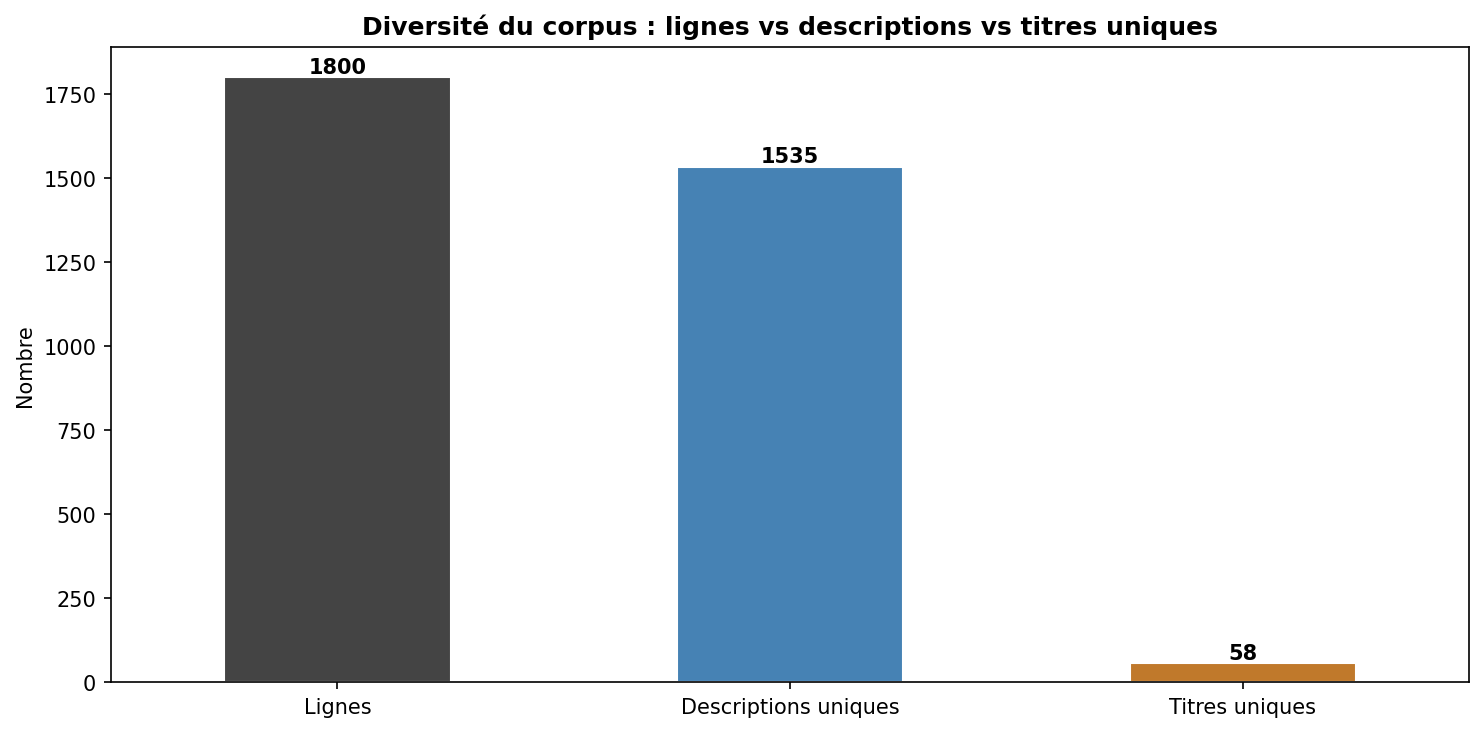
\includegraphics[width=0.90\textwidth]{ch03_redondance.png}
\caption{Diversité du corpus : lignes, descriptions et titres distincts}
\label{fig:redondance}
\end{figure}

Pour 1\,800 lignes, nous dénombrons 1\,535 descriptions distinctes, soit 85\,\% : à ce niveau, la
diversité est bonne. Les titres, eux, ne prennent que 58 valeurs distinctes, et le champ
\texttt{knowledge Base} en prend exactement autant. Le corpus s'organise donc autour de 58 types de
tickets récurrents, chacun instancié en moyenne 31 fois avec des variations de surface : demandeur,
dates, identifiants de configuration, tournures de phrase.

Cette structure a une conséquence directe sur le protocole expérimental. Un découpage aléatoire
entre entraînement et test placerait le même type de ticket des deux côtés. Le modèle retrouverait
au test un scénario déjà vu à l'entraînement, et le score mesuré refléterait sa capacité à mémoriser
plutôt qu'à généraliser. La section~\ref{sec:antifuite} traite ce risque.

\section{Diagnostic de qualité des données}

\subsection{Synthèse des indicateurs}

Le tableau~\ref{tab:dq} rassemble les indicateurs calculés dans les sections précédentes.

\begin{table}[!htbp]
\centering
\styletableau
\caption{Synthèse du diagnostic de qualité}
\label{tab:dq}
\begin{tabular}{|Bp{5.0cm}|Lp{3.6cm}|Lp{4.2cm}|}
\hline
\rowcolor{enteteTab}
\textbf{Indicateur} & \textbf{Valeur} & \textbf{Lecture} \\
\hline
Lignes et champs & 1\,800 sur 18 champs & Volume exploitable \\
\hline
Catégories & 8 & Classification multi-classes \\
\hline
Déséquilibre maximal & 5,93 & À traiter en modélisation \\
\hline
Tickets vides & 0 & Aucun \\
\hline
Doublons de ligne complète & 0 & Aucun \\
\hline
Incohérences d'étiquetage & 0 & Annotation fiable \\
\hline
Descriptions distinctes & 1\,535 sur 1\,800 & Diversité satisfaisante \\
\hline
Titres distincts & 58 & Corpus organisé par scénarios \\
\hline
Longueur des descriptions & médiane 33 mots & Textes homogènes \\
\hline
Champs critiques manquants & 0 & Complétude assurée \\
\hline
\end{tabular}
\end{table}

Le corpus est structurellement sain : aucune ligne vide, aucun doublon, aucune contradiction
d'étiquetage, et une complétude totale sur les champs essentiels. Ses difficultés portent sur la
forme de sa distribution et sur sa composition ; son intégrité, elle, est acquise.

\subsection{Risques identifiés et traitements retenus}

Le tableau~\ref{tab:risques} associe à chaque risque son effet attendu sur les modèles et le
traitement décidé, avec l'endroit du mémoire où ce traitement est mis en œuvre.

\begin{table}[!htbp]
\centering
\styletableau
\caption{Risques liés aux données et traitements associés}
\label{tab:risques}
\begin{tabular}{|Bp{2.9cm}|Lp{3.8cm}|Lp{4.2cm}|Cp{1.5cm}|}
\hline
\rowcolor{enteteTab}
\textbf{Risque} & \textbf{Effet attendu} & \textbf{Traitement} & \textbf{Où} \\
\hline
Déséquilibre des catégories & Rappel faible sur \emph{Sécurité} et \emph{Backup} & Métrique
F1-macro, pondération des classes, suivi du rappel par classe & Ch.~4 \\
\hline
Redondance des types de tickets & Fuite entre entraînement et test, scores surestimés & Découpage
par groupe de titres & \S\ref{sec:antifuite} \\
\hline
Nettoyage trop agressif & Perte de signal lexical, généralisation dégradée & Révision des règles,
conservation du vocabulaire informatique & \S\ref{sec:nettoyage} \\
\hline
Champs incomplets & Base de connaissances lacunaire & Repli de \texttt{Résolution/Motif} sur
\texttt{knowledge Base} & Ch.~5 \\
\hline
Données personnelles en clair & Exposition de noms et de rattachements & Non traité &
\S\ref{sec:rgpd} \\
\hline
\end{tabular}
\end{table}

\subsection{Limite assumée : la représentativité du corpus}
\label{sec:representativite}

Les deux sous-sections précédentes traitaient de risques que nous avons pu corriger. Celle-ci
énonce une limite que nous n'avons pas les moyens de lever. Le corpus décrit fidèlement l'activité
du service support d'\OTBS sur quatorze mois, et rien de plus.

Sa composition en 58 scénarios récurrents en délimite la portée. Un modèle entraîné sur ces données
apprend à reconnaître des familles de problèmes déjà rencontrées ; en revanche, ce corpus ne permet
pas de mesurer sa capacité à traiter un problème véritablement inédit, faute d'y trouver de tels
cas. Le rapprochement avec le jeu de données public conduit au même constat par un autre chemin :
91\,\% de titres uniques d'un côté, 3\,\% de l'autre. Les performances rapportées au chapitre~4
doivent se lire à cette échelle.

Le périmètre appelle deux restrictions supplémentaires. Le corpus couvre les huit entités du groupe
et leur parc applicatif, si bien que les résultats ne se transposent pas tels quels à une
organisation dont le paysage informatique diffère. Le référentiel de huit catégories, lui, est
propre au service : un autre découpage métier produirait un autre problème de classification. La
solution garde toute son utilité pour \OTBS, qui en est le destinataire ; ses chiffres, en
revanche, ne se généralisent pas.

\section{Préparation des données}

\subsection{Nettoyage textuel}
\label{sec:nettoyage}

Le nettoyage transforme le texte brut en une chaîne exploitable par les modèles. Il applique
successivement le passage en minuscules, la normalisation Unicode avec suppression des accents, le
retrait des adresses électroniques, des URL et des adresses IP, la suppression de la ponctuation, le
retrait des mots vides et le rejet des unités d'un seul caractère.

Notre première version de ces règles était trop agressive. Si elle figure ici, c'est parce qu'elle
illustre un piège courant. Elle retirait, en plus des mots vides du français et de l'anglais,
une longue liste de termes jugés génériques : \emph{problème}, \emph{système}, \emph{service},
\emph{demande}, \emph{ticket}. Le diagnostic a montré que la description moyenne tombait alors de
33 mots à une douzaine, et la diversité lexicale du corpus à environ 125 motifs distincts. Une
partie de l'uniformité que nous croyions lire dans les données venait en réalité du prétraitement
lui-même.

Nous avons donc révisé les règles. Une trentaine de termes informatiques discriminants sont
désormais protégés du retrait, qu'ils figurent ou non dans les listes de mots vides standard :
\emph{réseau}, \emph{serveur}, \emph{connexion}, \emph{outlook}, \emph{vpn}, \emph{dns},
\emph{sauvegarde}, \emph{sécurité}, entre autres. Les chiffres sont conservés, car un code d'erreur
ou un numéro de version porte de l'information ; seules les adresses IP restent retirées, trop
spécifiques pour se généraliser. La vectorisation retient enfin les unigrammes et les bigrammes, de
manière à capter des expressions comme \og salle serveur \fg{} ou \og tentatives connexion \fg{} que
le découpage en mots isolés dissout.

L'effet de cette révision sur les performances est mesuré au chapitre~4, sous le protocole qui y est
défini.

\subsection{Variables construites}

Nous ajoutons cinq variables aux dix-huit champs d'origine, ce qui porte le jeu préparé à
vingt-trois colonnes. Le tableau~\ref{tab:variables} les décrit.

\begin{table}[!htbp]
\centering
\styletableau
\caption{Variables construites lors de la préparation}
\label{tab:variables}
\begin{tabular}{|Bp{4.4cm}|Lp{4.2cm}|Lp{4.2cm}|}
\hline
\rowcolor{enteteTab}
\textbf{Variable} & \textbf{Construction} & \textbf{Destination} \\
\hline
\texttt{text\_clean} & Titre et description nettoyés & Vectorisation TF-IDF \\
\hline
\texttt{text\_enriched} & Préfixe de contexte, puis titre et description & Modèle CamemBERT \\
\hline
\texttt{text\_rag} & Titre, description, résolution et fiche de connaissance & Indexation du moteur
RAG \\
\hline
\texttt{priorite\_simple} & Quatre niveaux ramenés à trois & Contexte de classification \\
\hline
\texttt{classification\_simple} & Cinq types ramenés à trois & Contexte de classification \\
\hline
\end{tabular}
\end{table}

La variable \texttt{text\_enriched} demande un mot d'explication. Elle place devant le texte du
ticket un préfixe court de la forme \texttt{type demande priorite haute}, construit à partir des
deux variables simplifiées. L'idée est de donner au transformer un signal contextuel que le seul
texte libre ne porte pas toujours : une priorité élevée accompagne plus souvent les catégories
\emph{Infrastructure} et \emph{Sécurité} que \emph{Microsoft}. Le regroupement préalable des
modalités, de quatre à trois niveaux de priorité et de cinq à trois types, réduit le nombre de
préfixes possibles et limite la dispersion.

\subsection{Séparation anti-fuite}
\label{sec:antifuite}

La redondance mise en évidence plus haut impose un mode de découpage particulier. Le corpus
s'organisant en 58 types de tickets réinstanciés, un tirage aléatoire ligne à ligne placerait
presque à coup sûr chaque type des deux côtés de la séparation. Le modèle serait alors évalué sur
des scénarios qu'il a déjà vus, et le score obtenu ne mesurerait plus rien d'utile.

Nous regroupons donc les tickets par titre avant de tirer au sort, de sorte que tous les tickets
d'un même type restent du même côté. La figure~\ref{fig:split} oppose les deux approches.

\begin{figure}[!htbp]
\centering
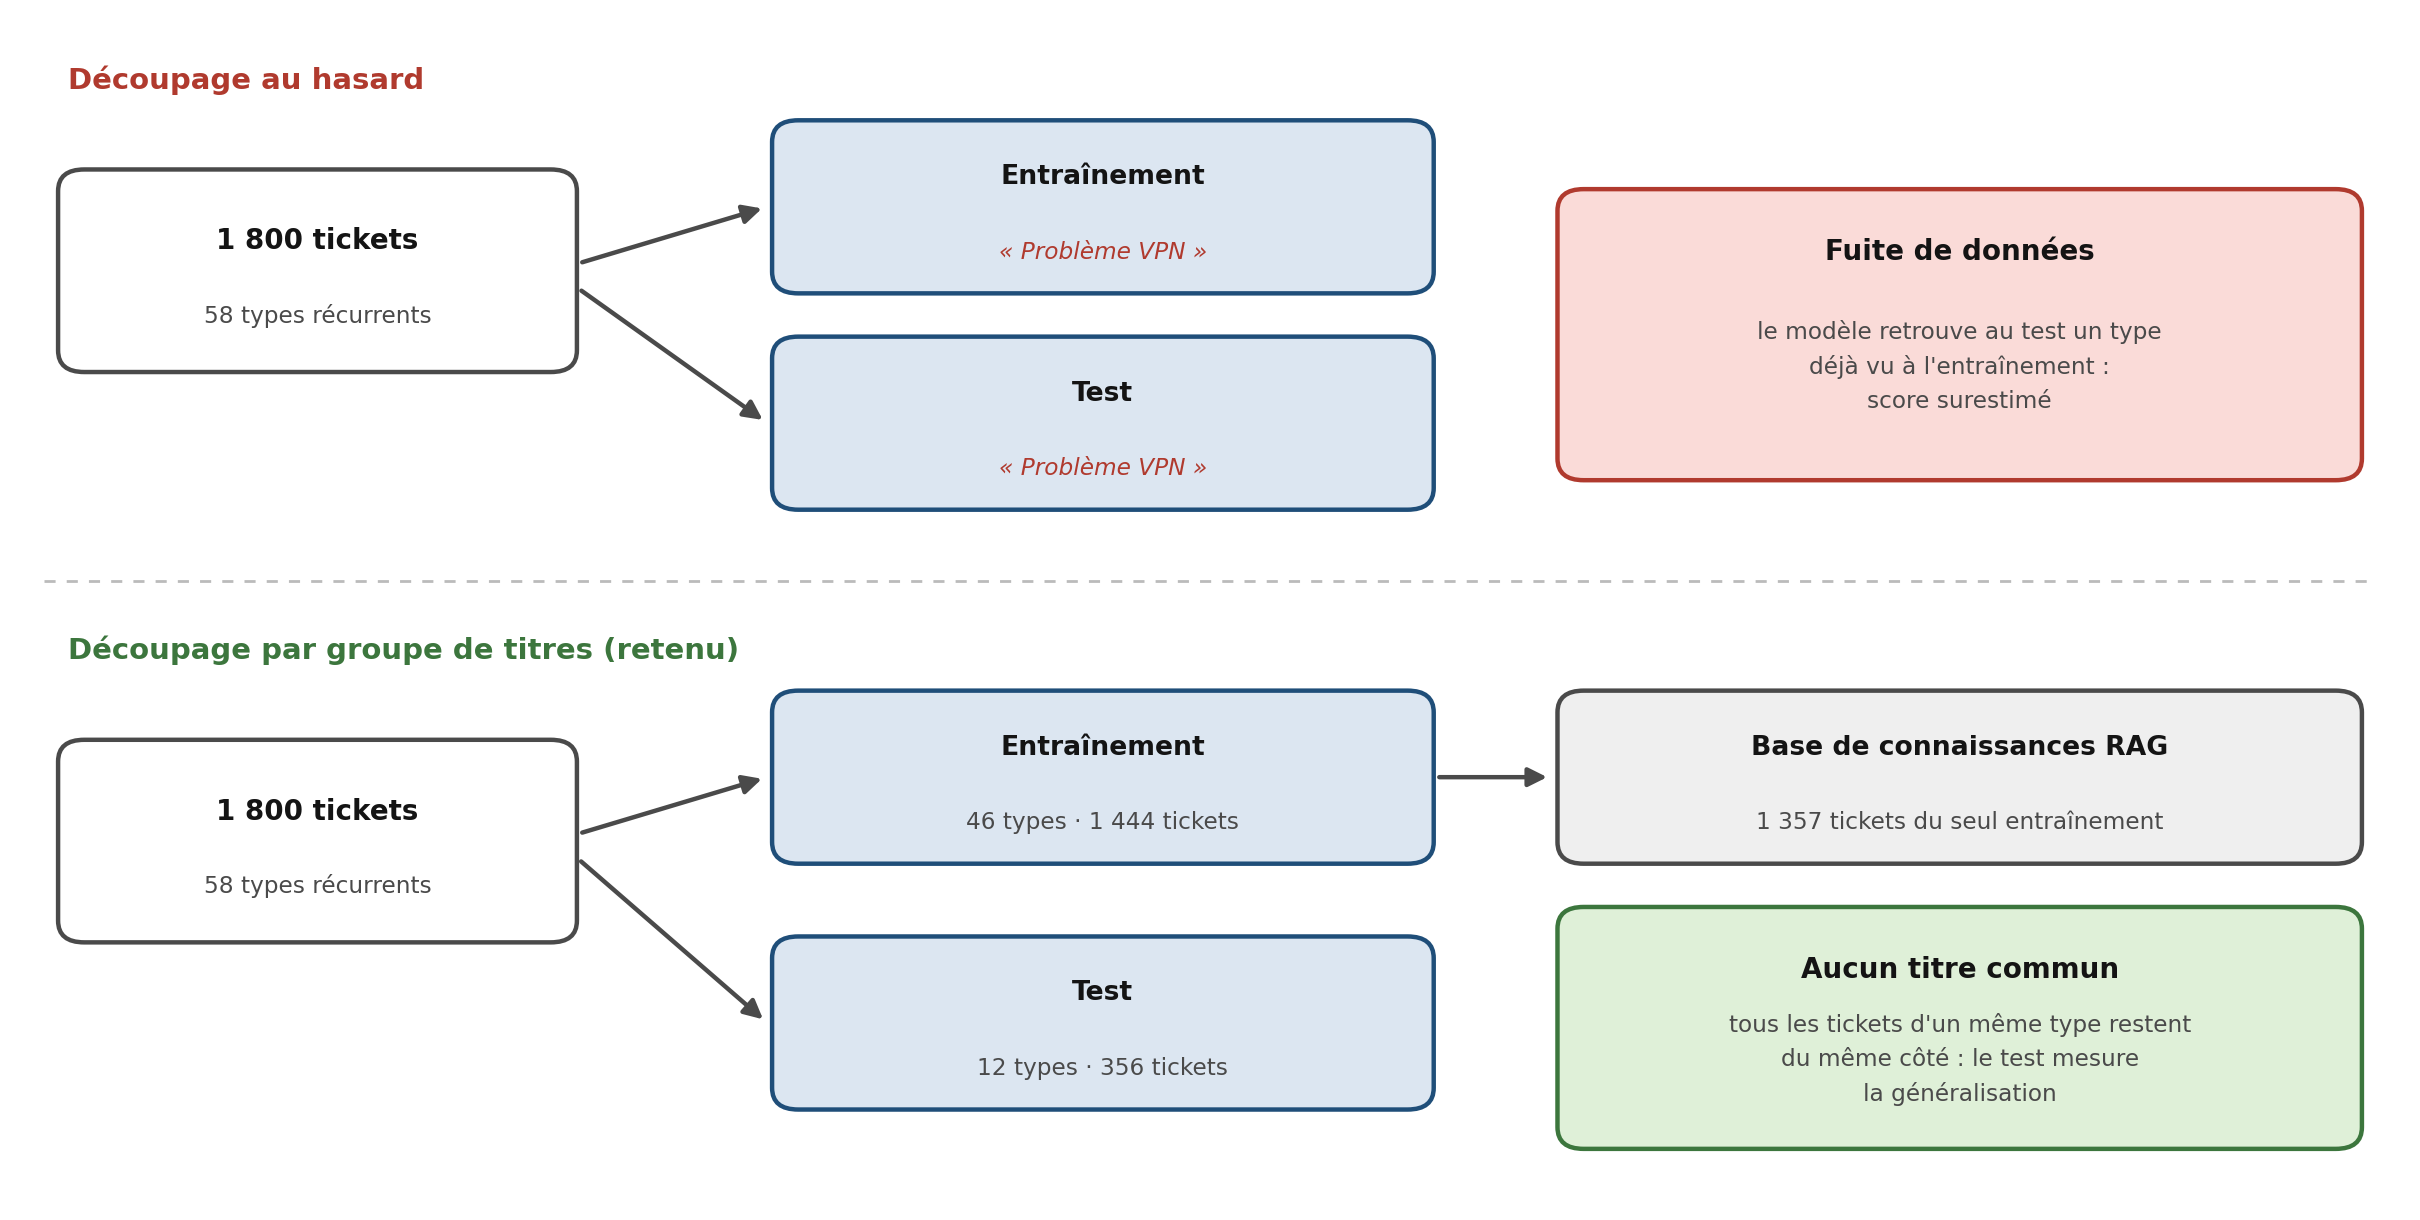
\includegraphics[width=\textwidth]{ch03_split_antifuite.png}
\caption{Découpage aléatoire et découpage par groupe de titres}
\label{fig:split}
\end{figure}

Le tirage est groupé, la colonne \texttt{Titre} servant de variable de groupe, avec une proportion
de test de 20\,\% et une graine aléatoire fixée pour la reproductibilité. Une assertion vérifie
après coup qu'aucun titre n'est commun aux deux jeux et interrompt le traitement dans le cas
contraire. Nous avons préféré cette vérification automatique à une relecture, qui n'aurait protégé
que la première exécution.

La base de connaissances du moteur RAG suit le même principe. Elle ne retient que des tickets du jeu
d'entraînement, ce qui empêche le moteur de retrouver la résolution d'un ticket de test au moment de
l'évaluation. Elle rassemble 1\,357 tickets : tous ceux du jeu d'entraînement
dont le champ \texttt{Résolution/Motif} est renseigné, quel que soit leur statut. Ce dernier point
s'écarte d'une intuition répandue, puisque la base ne se limite pas aux tickets résolus. Nous
l'assumons : un ticket rejeté documente une demande hors périmètre, un ticket en cours documente une
piste d'analyse, et l'un comme l'autre aident un consultant confronté à un cas voisin. La base se
répartit ainsi en 363 tickets rejetés, 358 résolus, 237 au statut \emph{Problème}, 236 pris en
charge et 163 en attente.

\subsection{Composition des jeux obtenus}
\label{sec:composition}

Le découpage produit 1\,444 tickets d'entraînement portant 46 types, et 356 tickets de test portant
les 12 types restants. Aucun titre n'est commun aux deux jeux : la fuite est éliminée.

Le tableau~\ref{tab:splits} donne la composition par catégorie et fait apparaître un effet
secondaire du procédé.

\begin{table}[!htbp]
\centering
\styletableau
\caption{Répartition des catégories dans les jeux obtenus}
\label{tab:splits}
\begin{tabular}{|Bp{3.4cm}|Cp{2.4cm}|Cp{2.2cm}|Cp{2.4cm}|}
\hline
\rowcolor{enteteTab}
\textbf{Catégorie} & \textbf{Entraînement} & \textbf{Test} & \textbf{Base RAG} \\
\hline
Microsoft & 274 & 135 & 263 \\
\hline
Réseau & 324 & 45 & 305 \\
\hline
Applicatifs & 326 & 0 & 303 \\
\hline
Infrastructure & 133 & 91 & 123 \\
\hline
Système & 134 & 52 & 128 \\
\hline
Communication & 144 & 0 & 133 \\
\hline
Sécurité & 40 & 33 & 36 \\
\hline
Backup & 69 & 0 & 66 \\
\hline
\rowcolor{enteteTab}
\textbf{Total} & \textbf{1\,444} & \textbf{356} & \textbf{1\,357} \\
\hline
\end{tabular}
\end{table}

Trois catégories sont absentes du jeu de test : \emph{Applicatifs}, \emph{Communication} et
\emph{Backup}. Le jeu de test ne couvre donc que cinq des huit catégories du référentiel.

Le procédé lui-même produit cet effet. Le tirage porte sur les titres, à l'exclusion des lignes, et
laisse libre la répartition des catégories qui en résulte. Les 12 types tirés au test relèvent
tous de cinq catégories seulement. Rien dans la mécanique du découpage groupé n'empêche cette
configuration, qui devient d'autant plus probable que le nombre de groupes est faible.

La conséquence est directe. Toute moyenne par catégorie calculée sur ce jeu de test porte sur cinq
classes et non sur huit. Le chiffre obtenu est mécaniquement supérieur à celui que donneraient les
huit catégories, puisqu'il exclut du calcul les classes rares, celles-là mêmes que le modèle traite
le moins bien. Les deux valeurs sont exactes ; seule leur comparaison est trompeuse. Le chapitre~4
rapporte donc ses résultats sous un protocole stratifié couvrant les huit catégories, et signale
explicitement les mesures issues du découpage groupé.

Ce constat justifie la réserve portée à l'objectif~4 au tableau~\ref{tab:obj3}. Le découpage remplit
bien la fonction pour laquelle nous l'avions conçu, l'élimination de la fuite ; il introduit en
revanche un biais que nous n'avions pas anticipé. La correction naturelle serait un découpage à la
fois groupé et stratifié, qui préserverait les groupes tout en équilibrant les catégories. Elle
figure parmi les perspectives de la conclusion générale.

\section{Gouvernance et reproductibilité}

\subsection{Versionnement des données et du pipeline}

La préparation décrite dans ce chapitre comporte plusieurs étapes enchaînées, dont les résultats
dépendent de paramètres numériques. Rejouée à la main, elle produirait tôt ou tard un jeu différent
de celui sur lequel les modèles ont été évalués, sans que nous puissions savoir lequel a servi à
quoi.

Nous décrivons donc le pipeline dans un fichier de configuration, exécuté par un outil de
versionnement de données. Le sprint en établit quatre étapes : le prétraitement du fichier brut, le
découpage en jeux, l'entraînement du modèle et la construction de l'index du moteur RAG. Chaque
étape déclare ses dépendances, ses paramètres et ses sorties. L'outil compare les empreintes de ces
éléments avant chaque exécution et ne rejoue que les étapes dont une entrée a changé. Le
chapitre~7 reprend ce même mécanisme et lui ajoute les étapes d'industrialisation.

Les paramètres sont centralisés dans un fichier unique : proportion de test, graine aléatoire,
nombre maximal de descripteurs de la vectorisation, seuils de confiance et de similarité. Les
changer revient à toucher une ligne de configuration plutôt que du code, et l'historique du dépôt
conserve la trace de chaque modification. Les fichiers de données eux-mêmes restent hors du dépôt de
code, remplacés par des empreintes qui permettent de retrouver la version exacte utilisée pour une
mesure donnée.

Le résultat est une garantie précise : chaque chiffre rapporté aux chapitres~4 et~5 se rattache à
une version identifiée des données et à un jeu de paramètres connu, et peut être recalculé à
l'identique.

\subsection{Données personnelles : une limite non traitée}
\label{sec:rgpd}

Le corpus contient des données à caractère personnel. Le champ \texttt{Demandeur} porte les noms de
202 collaborateurs, le champ \texttt{Assigné à} ceux des onze consultants, et le champ
\texttt{Filiale} rattache chaque personne à son entité. Les descriptions mentionnent par ailleurs
des identifiants de postes et de configurations.

Le diagnostic de qualité avait identifié l'anonymisation de ces champs comme une action prioritaire.
Nous ne l'avons pas réalisée. Les traitements décrits dans ce mémoire opèrent sur les données
nominatives telles qu'exportées.

Le manquement est réel, même si deux circonstances en limitent la portée. L'ensemble de la chaîne
s'exécute sur l'infrastructure d'\OTBS, sans transmission vers un service extérieur : l'exigence de
confidentialité posée dès le chapitre~1 est respectée. Et les modèles se nourrissent du seul titre,
de la description et des champs de résolution ; les champs nominatifs restent à l'écart du
traitement. Cela ne nous exonère pas pour autant. Remplacer les noms par des identifiants stables
au moment du chargement aurait coûté peu et supprimé le risque à la source. Le point figure parmi les travaux à conduire
avant tout déploiement élargi.

\section{Bilan du sprint}

Le sprint livre un jeu de données décrit, mesuré, nettoyé, découpé et versionné, ainsi qu'un
diagnostic de qualité qui documente ce que le corpus permet d'établir et ce qu'il ne permet pas.
Les objectifs 1, 2, 3 et 5 sont atteints sans réserve. L'objectif~4, le découpage anti-fuite, l'est
avec la restriction analysée à la section~\ref{sec:composition}.

Trois acquis conditionnent la suite. Le protocole de découpage fixe le cadre d'évaluation de tous
les modèles comparés au chapitre~4. La base de connaissances de 1\,357 tickets fournit la matière du
moteur de recherche construit au chapitre~5. Le troisième est moins visible : le diagnostic de
représentativité, qui détermine par avance l'échelle à laquelle il faudra lire les résultats des
deux chapitres suivants.

\section*{Conclusion}
\addcontentsline{toc}{section}{Conclusion}

Le corpus réuni compte 1\,800 tickets couvrant quatorze mois d'activité, répartis en huit catégories
et décrits par dix-huit champs. Son intégrité est bonne et son annotation cohérente ; les champs
exploités par les modèles sont renseignés partout.

Ses difficultés se situent ailleurs. La distribution des catégories est inégale d'un facteur 5,93,
et le corpus s'organise autour de 58 types de tickets récurrents plutôt qu'autour de problèmes tous
distincts. Le chapitre~4 traite la première, par le choix de la métrique et par la pondération. La
seconde nous a conduits au découpage par groupe de titres : il élimine bien la fuite visée, mais il
laisse trois catégories hors du jeu de test, limite énoncée ici et dont le protocole du chapitre
suivant tient compte.

Le chapitre~4 exploite ces jeux pour comparer plusieurs approches de classification, d'une
vectorisation classique à l'adaptation d'un transformer francophone, et pour analyser les écarts
entre les résultats obtenus et les objectifs fixés au démarrage du projet.
